
\chapter{Implementation}

\section{Tools}

The programming language chosen to implemented the system was c++.
The arguments leading to this choice was:

\begin{itemize}
\item Most of the group members had some earlier experience with the language.
\item It allows for a high level of abstraction without loosing control of the
underlying hardware.
\item The code can be easily parallelized for shared memory machines using OpenMP.
\item Many libraries exist for c++ that implements highly optimized linear algebra
functionality.
\end{itemize}

Other languages cosidered where Matlab and c.

The tool chosen to visualize the resulting data was gnuplot and ffmpeg. Writing a
program using OpenGL was considered, but dismissed on the grounds of beeing too time consuming.

\section{Program design}

\begin{figure}[!h]
  \begin{center}
    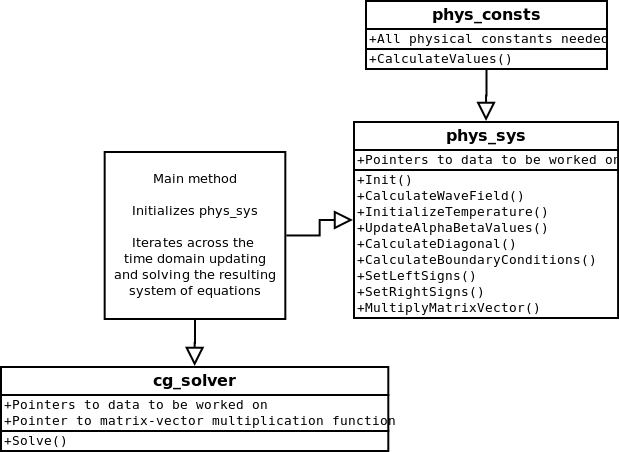
\includegraphics[width=0.5\linewidth]{classdiagram.png}
  \end{center}
  \caption{Class diagram of c++ implementation}
  \label{fig:classdiagram}
\end{figure}

The program mainly consist of three parts:

\begin{itemize}
\item C++ implementation of Linear algebra functionality of the discrete equations.
\item C++ implementation of the conjugate gradient method for solving the
equations described.
\item Bash script for generating plots and and movie of the generated data.
\end{itemize}

See \cref{fig:classdiagram} for a class diagram of c++ implementation.

The Bash script is not discussed in further detail as it can be considered to be
very simple.

See \cref{ap:source_code} for source code and scripts.

\section{The physical system}

The main task of the physical system is to implement a matrix-vector multiplication
procedure for the heat equation to be used in the conjugate gradient method, 
a method for calculating the heating properties of the microwave and a method 
for calculating the velocity of mass transfer.

\subsection{Partitioning of the problem}

The problem is to perform the multiplication of a sparse, symmetrix, matrix with a
vector. To describe this procedure we have vectors $a$, $b$ and $t$ containing alpha,
beta, and temperature values respectively. The alpha values represent the heat 
conduction properties, the beta values describe the substance's ability to be heated
by microwaves and the temperature values naturally contains the temperatures. We need
these vectors because each point in the grid contains a particular substance in
a particular phase.

\begin{figure}[!h]
  \begin{center}
    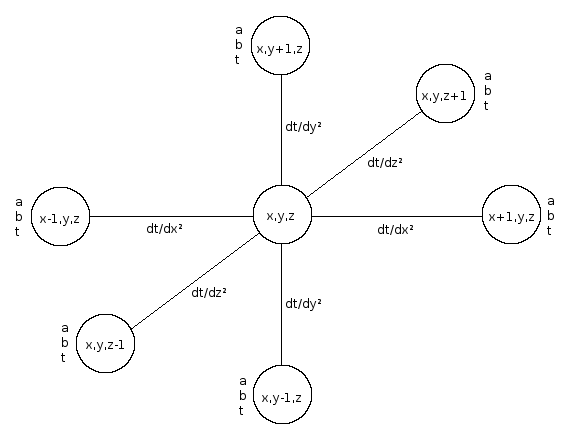
\includegraphics[width=0.5\linewidth]{stencil.png}
  \end{center}
  \caption{Stencil}
  \label{fig:stencil}
\end{figure}

\begin{figure}[!h]
  \begin{center}
    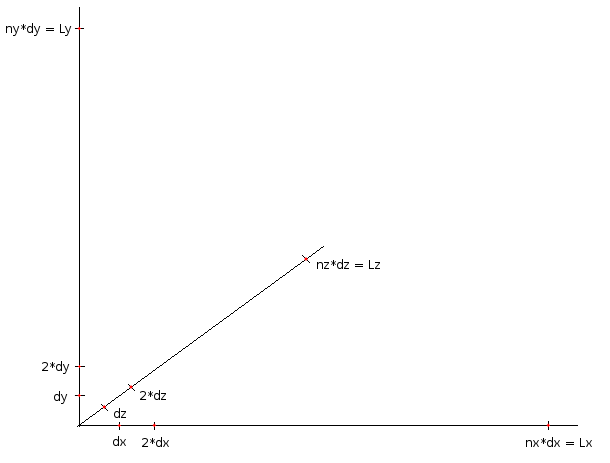
\includegraphics[width=0.5\linewidth]{grid.png}
  \end{center}
  \caption{Grid}
  \label{fig:grid}
\end{figure}

We say that position $j$ of the vectors is given by:
\begin{equation}
j = z*n_x*n_y + y*n_x + x
\end{equation}

where $n_x$, $n_y$, $n_z$ is the number of points in the $x$, $y$ and $z$ directions
respectively, and $x$, $y$ and $z$ is the points on the grid, See \cref{fig:grid} and
\cref{fig:stencil}

The center of the stencil, given by $j$ can be described by the equations:
\begin{eqnarray}
  x & \cong & j\%n_x \\
  y & \cong & (j/n_x)\%n_y \\
  z & \cong & j/n_x/n_y 
\end{eqnarray}

where $/$ and $ \% $ is the integer division and modulo operators respectively.

In addition to this, we define two more vectors and one more matrix:

The offset matrix represents the neighbours in the stencil (see \cref{fig:stencil}):
\begin{equation}
O =
\left[
\begin{array}{ccc}
0 & 0 & -1 \\
0 & -1 & 0 \\
-1 & 0 & 0 \\
0 & 0 & 0 \\
1 & 0 & 0 \\
0 & 1 & 0 \\
0 & 0 & 1 \\
\end{array}
\right]
\end{equation}

The delta vector representing the difference in time and distance used in the heat
equation:
\begin{equation}
D = \{ \frac{dt}{dz^2}, \frac{dt}{dy^2}, \frac{dt}{dx^2}, 0, \frac{dt}{dx^2}, \frac{dt}{dy^2}, \frac{dt}{dz^2} \}
\end{equation}

The vector containing the offsets relative to the diagonal in the matrix we are multiplying
with:
\begin{equation}
R = \{ -n_x*n_y, -n_x, -1, 0, 1, n_x, n_x*ny \}
\end{equation}

Note that the indexing of these vectors and matrices correspond, so by looping through them,
We have all the information we need to perform the necessary operations.

\subsection{Updating alpha and beta values}

When updating the alpha and beta values, we simply loop through the temperature
vector, and update the alpha and beta vectors to their correct values using the
physical contants describing the substance at that point.

\subsection{Calculating the distribution of the microwave effect}

This is done according to \cref{eq:effektfordeling} and by multiplying the
resulting distribution by the microwave effect and dividing by the volume at each point
in the grid.

\subsection{The matrix-vector multiplication procedure}

The matrix-vector multiplication procedure takes advantage of the fact that our 
matrix is sparse and that our problem is well defined. Thus, the algorithm used
will complete in $m$ iterations where $m$ is the number of non-zero entries in 
the matrix. $m$ is approximately equal to $7*n$.

\section{The conjugate gradient method as an iterative algorithm}

The method (conjugate gradient) used to solve the system of equations is based on 
the steepest descent algorithm, however, it results in the exact solution within
$n$ iterations. This is, however, assuming we have infinite floating point accuracy.

The iterative conjugate gradient method lets us define an acceptable error, and stops
once our solution has an error below what is acceptable.

In our implementation, we recompute the correct residual to avoid accumulation of
floating point precision errors, however, this is not done at each iteration, and may
result in the need of more than $n$ iterations for the algorithm to complete.

\section{The main procedure}

\begin{itemize}
  \item Initialize problem; define grid-size, dimensions of bacon, partitioning of fat vs meat
  and internal and external temperature.
  \item Allocate necessary memory
  \item Initialize physical system
  \item Initialize internal temperature
  \item Initialize internal flow
  \item Calculate boundary conditions
  \item Calculate micro-wave field
  \item Initialize conjugate gradient solver
  \item loop
  \begin{itemize}
    \item Update alpha and beta values
    \item Calculate diagonal
    \item Set signs for right side multiplication (t=n)
    \item Multiply right side of heat equation
    \item Add micro-wave effect to right side of equation
    \item Set signs for left side of equation (t=n+1)
    \item Solve using conjugate gradient method
  \end{itemize}
\item Deallocate memory
\end{itemize}

\section{Parallel speedup}

The program was tested with $n_x=n_y=n_z=15$ giving $n=n_x*n_y*n_z=3375$ and $n_t=100000$.

The sequantial version of the program ran in 342 seconds. 
The parallel version ran in 194 seconds (2 cores) and 181 seconds (4 cores).

This gives us a speedup of:
\begin{equation}
S_p(2) = \frac{T_s}{T_{p,2}} = \frac{342}{194} = 1.76
\end{equation}

and

\begin{equation}
S_p(4) = \frac{T_s}{T_{p,4}} = \frac{342}{181} = 1.89
\end{equation}

The reason the speedup between 2 and 4 cores was so small may be due to a lack of
parallelizable work. The code can only be parallelized on the spacial work ($n$) of the
heat equation, and not across the time domain ($n_t$). Thus, most of the work involved in
this program is sequential.

The conjugate gradient method is not parallelizable either (except for the linear algebra functions it
uses). Thus, the total of parallelizable work is just $n$, which for this example may be too small.

\section{Unimplemented functionality}

Due to timeconstraints and unforeseen complications, the flow equations was not implemented, 
however a significant amount of effort was put into the implementation before it was 
abandoned.

The numerical schemes implemented in an attemt at solving the equations was:

\begin{itemize}
  \item Forward euler
  \item Runge-Kutta
\end{itemize} 

Forward euler was dismissed as the difference in time had to be too small to be practical.

The runge kutta method also gave us some strange and unforeseen results.

After looking closely at the differential equations and their discrete equivelents, a number
of practical issues surfaced. And the continued development of the equations was dismissed
as the project was close to its end.


